\documentclass{ximera}
\typeout{Start loading xmPreamble.tex}%

% Extra macros loaded automatically by all documents of class 'ximera' or 'xourse'

\newcommand{\PP}{\mathbb{P}}
\newcommand{\EE}{\mathbb{E}}
\newcommand{\Var}{\mathrm{Var}}
\newcommand{\indep}[2]{\PP\left(#1 \cap #2\right) = \PP\left(#1\right) \cdot \PP\left(#2\right)}
\newcommand{\cond}[2]{\frac{\PP( #1 \cap #2)}{\PP(#2)}}
\newcommand{\pdf}{\text{probability distribution function}}

% Ximera already defines theorem-like environments:
% theorem, lemma, corollary, example, definition, etc.
% So do NOT redefine them here.

\usepackage{tikz}
\usetikzlibrary{positioning, arrows.meta}

\usepackage{multicol}
\usepackage{enumitem}
\usepackage{caption}
\usepackage{amsmath,amssymb,amsfonts}
\usepackage{mathtools}
\usepackage{graphics}
\usepackage[T1]{fontenc}
\usepackage{colortbl}
% \usepackage{fouriernc}
\usepackage{marvosym}
\usepackage{color}

\providecommand{\Lightning}{\ensuremath{\text{\sffamily\bfseries !}}}

\def\arrvline{\hfil\kern\arraycolsep\vline\kern-\arraycolsep\hfilneg}

\title{Chapter 2}
\begin{document}
\begin{abstract}
\end{abstract}
\maketitle
\section{Chapter 2}

\subsection{Counting arguments}
So far in the last two weeks, we have seen Kolmogorov's axioms for probability, and some formulas to calculate the probability of events. We'll move into chapter 2 of the textbook, which covers discrete random variables. One of the examples is the binomial distribution, which requires understanding what binomials are. Because this is not covered under the required prerequisites, I won't assume you've seen it before. I will discuss them in a probability context (using the total probability rule), so you'll see something new even if you've already learned about binomials already. \footnote{This is actually a simple example of a branch of math called probabilistic combinatorics, which uses probability methods towards combinatorial problems.}

The main points are:

\begin{definition}
The \textit{binomial} $\binom{n}{k}$ is defined to be
$$
\binom{n}{k} = \frac{n!}{k! (n-k)!}.
$$
It counts the number of ways to pick $k$ objects from a collection of $n$ identical objects, where the order of the objects does not matter.  The \textit{binomial theorem} states that
$$
(x+y)^n = \sum_{k=0}^n \binom{n}{k} x^k y^{n-k}.
$$
\end{definition}

First, we will see that $n!=n(n-1)\cdots 1$ is the number of ways to arrange $n$ distinct items. For example, suppose we want to know how many ways there are to arrange $5$ cards, numbered $1,2,3,4,5$. If we shuffle the cards enough times, we'll have a uniform probability law on the set $\Omega$ of all possible arrangements. A uniform probability law takes the same value on each outcome, so the probability of finding each arrangement is $1/\vert \Omega\vert$. So to find the total number of arrangements, we can find the probability of a single arrangement, and then take its inverse. For simplicity, let's find the probability of the arrangement where the top card is $1$, the second card is $2$, and so on. Let's write this as $\PP( (1,2,3,4,5))$. By the multiplication rule, 
\begin{multline*}
\PP((1,2,3,4,5)) = \PP(\text{top card is 1}) \cdot \PP(\text{second card is 2} \vert \text{top card is 1}) \cdot \PP(\text{third card is 3} \vert \text{top two cards are }(1,2)) \\
\cdot \PP(\text{fourth card is 4} \vert \text{top three cards are } (1,2,3)) \cdot \PP(\text{last card is 5} \vert \text{ top four cards are } (1,2,3,4)).
\end{multline*}
It should be straightforward to see that this equals
$$
\frac{1}{5} \cdot \frac{1}{4} \cdot \frac{1}{3} \cdot \frac{1}{2} \cdot \frac{1}{1} = \frac{1}{5!}.
$$
Therefore, there are $5!$ ways to arrange these $5$ cards. In general, there are $n!$ ways to arrange $n$ distinct objects. 

Second, we will see that the number of ways to pick $k$ items out of $n$ total (where the order matters) is $n!/(n-k)!$. Notice that when $k=n$, this is just $n!$. Picking $n$ items out of $n$ total means that you're just re-arranging the $n$ items. As an example, suppose that you have $7$ cards numbered $1,2,3,4,5,6,7$ and you want to pick $3$ of them. The order of them matters, so $(6,1,4)$ is different than $(6,4,1)$. We can use the same ideas as before: shuffle the cards enough and you have a uniform probability law $\PP$. By the multiplication rule,
$$
\PP((1,2,3)) = \PP(\text{top card is 1}) \cdot \PP(\text{second card is 2} \vert \text{top card is 1}) \cdot \PP(\text{third card is 3} \vert \text{top two cards are }(1,2)),
$$
which equals 
$$
\frac{1}{7} \cdot \frac{1}{6} \cdot \frac{1}{5} = \frac{4!}{7!} = \frac{(7-3)!}{7!}.
$$
In general, the formula is $n!/(n-k)!$.

Finally, we'll ask how many ways there are to pick $k$ items out of $n$ total (where the order doesn't matter). It turns out to be exactly $\binom{n}{k}$. Repeating the same argument as above, where $(1,2,3),(1,3,2),(2,1,3),(2,3,1),(3,1,2),(3,2,1)$ are all the same hand (like in a poker game), then we have
$$
\PP({1,2,3}) = \PP((1,2,3))+\PP(1,3,2))+\mathbb{P}((2,1,3))+\mathbb{P}((2,3,1))+\mathbb{P}((3,1,2))+\mathbb{P}((3,2,1)).
$$
From the previous example, we're adding the quantity $(7-3)!/7!$ to itself $3!$ times, so we get $(7-3)!3!/7!$, which is the inverse of $\binom{7}{3}$. In general, we would be adding $(n-k)!/n!$ to itself $k!$ times (because there are $k$ ways to rearrange out hand of $k$ cards), so the general formula is $\binom{n}{k}$.

How does the binomial relate to the binomial theorem? Suppose we want to expand $(x+y)^7$. We could try to use the distributive property to multiply
$$
(x+y)(x+y)(x+y)(x+y)(x+y)(x+y)(x+y),
$$
but that would take too long. Let's say we wanted to find the coefficient of $x^3y^4$. Each possible way to pick $3$ cards from a deck of $7$ cards corresponds to the coefficient of $x^3y^4$. For example, if we've picked the cards $\{6,1,4\}$, this corresponds to 
$$
({\color{pink}x}+y)(x+{\color{brown}y})(x+{\color{brown}y})({\color{pink}x}+y)(x+{\color{brown}y})({\color{pink}x}+y)(x+{\color{brown}y}).
$$
There are $\binom{7}{3}$ ways to pick $3$ cards out of $7$, so the coefficient of $x^3y^4$ is $\binom{7}{3}$.  More generally, the coefficient of  $x^ky^{n-k}$ in $(x+y)^n$ is $\binom{n}{k}$.  This is exactly the binomial theorem.

\subsection{Discrete Random Variables}

We'll now move into the chapter on discrete random variables. First, we'll need to define what a random variable is. Later, we'll get to several important examples of discrete random variables (Bernoulli, Binomial, Geometric, Poisson), that occur frequently in probability theory. 

\begin{definition}
A random variable is a function $X$ from $\Omega$ to some subset of $\mathbb{R}$. If the image of $X$ is discrete, we call it a discrete random variable. If the image of $X$ is continuous, we call it a continuous random variable.
\end{definition}

For example, let's say we flip a coin (fair or not, independently or not) seven times. The number of heads we get is a random variable. The sample space $\Omega$ is $\{H,T\}^{\times 7}$, and $X$ is a function from $\Omega$ to $\{0,1,2,3,4,5,6,7\}$. For example,
$$
X(\text{HHTHTTT})=3.
$$

In the previous example, the random variable $X$ is defined without referencing $\PP$. In order to say something interesting about a random variable $X$, we have to relate it to the probability law on $\PP$ on $\Omega$. This is done through something called the probability mass function.

\begin{definition}
The \textit{probability mass function} (PMF) of a random variable $X$ is the function $p_X$ defined by
$$
p_X(n) = \mathbb{P}(X^{-1}(n)).
$$
This will more commonly be written as $p_X(n) = \PP(X=n)$.
\end{definition}
You read this as:
\begin{center}
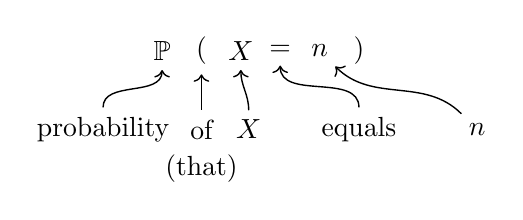
\begin{tikzpicture}
\node at (0,0) (aa)  {$\PP$};
\node at (0.5,0) (bb) {$($};
\node at (1,0) (cc)  {$X$};
\node at (1.5,0) (dd)  {$=$};
\node at (2,0) (ee)  {$n$};
\node at (2.5,0)  {$)$};
\node at (-0.75,-1) (a) {probability};
\node at (0.5,-1) (b) {of};
\node at (1.1,-1) (c) {$X$};
\node at (2.5,-1) (d) {equals};
\node at (0.5,-1.5) {(that)};
\node at (4,-1) (e) {$n$};
\draw (aa) edge[out=-90,in=90,<-, line width=0.5pt] (a);
\draw (bb) edge[out=-90,in=90,<-, line width=0.5pt] (b);
\draw (cc) edge[out=-90,in=90,<-, line width=0.5pt] (c);
\draw (dd) edge[out=-90,in=90,<-, line width=0.5pt] (d);
\draw (ee) edge[out=-45,in=135,<-, line width=0.5pt] (e);
\end{tikzpicture}
\end{center}

\subsubsection{Bernoulli Random Variable}
Here is the most basic example of a discrete random variable, called the Bernoulli\footnote{Trivia about Jacob Bernoulli: his parents made him study philosophy and theology, which he resented. After earning a master's degree in philosophy in 1671 and a licentiate in theology in 1676 from the University of Basel (in Switzerland), he became a mathematician.} random variable.

\begin{definition}
A random variable $X$ is called a \textit{Bernoulli random variable} if its probability mass function is
$$
p_X(n)
= 
\begin{cases}
p, & \text{ if } n=1,\\
1-p, & \text{ if } n=0.
\end{cases}
$$
We denote this as $\text{Ber}(p)$.
\end{definition}

There are a few natural ways that Bernoulli random variables occur. For example, consider a game between Texas A\&M and Alabama, where Texas A\&M wins with probability $p$. (Assume there are no ties). Then the sample space is
$$
\Omega = \{W,L\}
$$
and define the random variable $X$ to be $1$ for a win and $0$ for a loss. Then $X$ is a Bernoulli random variable. We write this as $X \sim \text{Ber}(p)$ or $X\stackrel{d}{=} \text{Ber}(p)$. An Alabama fan, on the other hand, might define a random variable $Y$ to be $1$ for an Alabama win and $0$ for an Alabama loss. Then $Y \sim \text{Ber}(1-p)$.

Another example might come from running an experiment (these are sometimes called Bernoulli trials). If the experiment is a success with probability $p$ and a failure with probability $1-p$, then
$$
\Omega = \{\text{success}, \text{failure}\}.
$$
If $Z$ is $1$ for a success and $0$ for a failure, then $Z\sim \text{Ber}(p)$.

We note that different random variables can be defined on the same sample space $\Omega$, depending on your perspective (e.g. which team you're rooting for). Also note that two random variables with the same PMF can be defined on different sample spaces. This is why we write $X \sim \text{Ber}(p)$ or $X\stackrel{d}{=} \text{Ber}(p)$ instead of just $X = \text{Ber}(p)$.

Question: what is the PMF of $X+Y$? Does $Y+Z$ make sense? If we tried to write $Y=\text{Ber}(p)$ and $Z= \text{Ber}(1-p)$, how might the notation mislead us?

\subsubsection{Binomial Random Variable}
The next example of a discrete random variable is a binomial random variable:

\begin{definition}
A random variable $X$ is called a \textit{binomial random variable} if its probability mass function is
$$
p_X(k) = \binom{n}{k} p^k (1-p)^{n-k}, \text{ for } k=0,1,\ldots,n.
$$
We denote this as Binom$(n,p)$.
\end{definition}

The binomial random variable comes up in the following setting. Suppose that two teams play series of $n$ games each other (let's call the teams Texas A\&M and Auburn). Let $X$ denote the number of games that Texas A\&M wins. If Texas A\&M has a probability $p$ of winning each game, and all games are independent, what is the probability mass function of $X$?

Let's consider an example where $n=5$ and $k=3$. One way to win three games is to win the first, second and fourth games, while losing the third and fifth. Because the games are independent, we have
\begin{align*}
\PP(\text{WWLWL}) &= \PP(\text{win first}) \cdot \PP(\text{win second}) \cdot \PP(\text{lose third}) \cdot \PP(\text{win fourth}) \cdot \PP(\text{lose fifth})\\
&= \hspace{0.3in} p \hspace{0.7in} p \hspace{0.7in} (1-p) \hspace{0.7in}  p \hspace{0.5in}  (1-p)\\
&= p^3(1-p)^2.
\end{align*}
Of course, there are other ways in win three games. For example, one way is to win the second, fourth and fifth. As we saw in the section on counting methods, there are $\binom{5}{3}$ total ways. So $p_X(3) = \binom{5}{3}p^3(1-p)^2$. For $n$ games total, we have $p_X(k) = \binom{n}{k} p^k (1-p)^{n-k}$; in other words, $X\sim \text{Binom}(n,p)$. 

\subsubsection{Geometric Random Variable}
So far, we've seen examples of discrete random variables supported on finite values. The next two examples can take values on the entire set of natural numbers, $\mathbb{N}=\{0,1,2,\ldots\}$.
\begin{definition}
A random variable $X$ is a \textit{geometric} random variable if its probability mass function is
$$
p_X(k) = (1-p)^k p \text{ for } k=0,1,2,3,\ldots
$$
We denote this Geo$(p)$.
\end{definition}

Here is the usual example of a geometric random variable. Suppose that two teams are playing against each other. Let's call them ... Texas A\&M and LSU. Assume that all games are independent, and Texas A\&M wins with probability $p$. Let's say that they'll keep playing until Texas A\&M gets a win, because ``Aggies cannot stand to lose''\footnote{\url{https://www.tamu.edu/traditions/remembrance/muster/}}. Let $X$ be the number of losses that Texas A\&M has. What is the probability mass function of $X$? 

Well, if Texas A\&M loses $k$ games, then we're looking at the probability of the sequence $\underbrace{LL \cdots L}_{k}W$. Since all games are independent, this has probability $(1-p)^kp$, so $X\sim \text{Geo}(p)$.

Recall (from calculus) that a geometric series is a series of the form
$$
1+q+q^2 + \ldots = \frac{1}{1-q}, \text{ for } -1<q<1,
$$
hence the name geometric random variable (from setting $q=1-p$).

\subsubsection{Poisson Random Variable}
The last example we'll give is the Poisson\footnote{Trivia about Sim\'{e}on Denis Poisson (1781--1840): his last name literally means ``fish'' in French, and his name is inscribed on the Eiffel tower.} random variable.

\begin{definition}
A random variable $X$ is called a \textit{Poisson} random variable if its probability mass function is
$$
p_X(n) = e^{-\lambda} \frac{\lambda^n}{n!}.
$$
We denote it as $X\sim \text{Pois}(\lambda)$.
\end{definition}

The previous random variables had straightforward examples. The Poisson random variable is actually a little tricker. It models events that occur rarely and independently. Examples would include accidents, or asteroids hitting the earth. The most famous example comes from Ladislaus Bortkiewicz, who published the book ``The Law of Small Numbers'' in 1898 with data suggesting that the number of Prussian soldiers kicked to death by a horse is a Poisson random variable. It is somewhat interesting that Poisson developed the formula for a Poisson random variable before anyone demonstrated that it could occur in the real world. 

So suppose that on \textit{average}, $\lambda$ accidental horse-kick deaths occur in a year. Let $X$ be the number of death in a year. What is the probability mass function of $X$?

We model the year as 365 \textit{independent} Bernoulli trials. (Question: does it actually make sense to say these are independent?) The ``success'' rate is then $p=\lambda/365$. So we can approximate $X$ by a $\text{Binom}(365,\lambda/365)$ random variable:
$$
p_X(k) \approx \binom{365}{k} \left( \frac{\lambda}{365}\right)^k \left( 1- \frac{\lambda}{365}\right)^{365-k}.
$$ 
Because $365\approx \infty$, we can make the approximation
$$
p_X(k) \approx \lim_{n\rightarrow\infty} \binom{n}{k} \left( \frac{\lambda}{n}\right)^k \left( 1- \frac{\lambda}{n}\right)^{n-k}.
$$
This approximation only works if the events rarely occur (because we're taking the ``success'' rate $\lambda/n$ to be close to $0$).

How do we calculate this limit? The ``trick'' is to take the definition of the exponential function and its Taylor series:
$$
e^x = \lim_{n\rightarrow \infty} \left( 1 + \frac{x}{n}\right)^n = \sum_{k=0}^{\infty} \frac{x^k}{k!}.
$$
By the binomial theorem,
$$
\lim_{n\rightarrow\infty} \sum_{k=0}^n \binom{n}{k} 1^{n-k} \left( \frac{x}{n}\right)^k = \sum_{k=0}^{\infty} \frac{x^k}{k!}
$$
By comparing the $x^k$ coefficient, we see that
$$
\lim_{n\rightarrow \infty} \binom{n}{k} \frac{1}{n^k} = \frac{1}{k!}.
$$
We plug this in to get that
\begin{align*}
p_X(k) &\approx \lim_{n\rightarrow\infty} \binom{n}{k} \left( \frac{\lambda}{n}\right)^k \left( 1- \frac{\lambda}{n}\right)^{n-k} \\
&= \binom{n}{k} \frac{1}{n^k} \lambda^k \left( 1- \frac{\lambda}{n}\right)^{n} \left( 1- \frac{\lambda}{n}\right)^{-k}\\
&= \frac{\lambda^k}{k!} e^{-\lambda},
\end{align*}
which is the Poisson PMF.

\Lightning \Lightning This is a common method in probability, where we ``transform'' a problem about probability to a problem about series or functions. We'll see this more in chapters 4 and 5. \Lightning \Lightning

\subsubsection{{\color{lime} Optional: Negative Binomial Random Variable}}
Suppose we run independent Bernoulli trials, where the probability of success if $p$ and failure is $(1-p)$. We observe these trials until $r$ failures have occurred. Let $X$ denote the number of successes. Then
$$
p_X(k) = \binom{k+r-1}{k} (1-p)^r p^k,
$$
and we say $X$ is distributed as the negative binomial distribution; $X\sim \text{NB}(r,p)$. The negative binomial distribution is sometimes a better model than the Poisson distribution. Part of the benefit is that the negative binomial distribution has two parameters instead of just one. 

The parameter $r$ can take non--integer values, but this requires understanding the factorial through something called the Gamma function $\Gamma$, which we will not go into. For example,
$$
\left( \frac{1}{2}\right)! = \frac{\sqrt{\pi}}{2}
$$

\subsection{Some properties of probability mass functions}
We'll note some properties of PMFs:
$$
\sum_n p_X(n) = 1
$$
and 
$$
p_X(n) \geq 0 \text{ for all } n.
$$

\newpage



\subsection{Expected Value}
In the example of the Poisson random variable, we saw that the average number of incidents was $\lambda$. We will need a mathematical definition of ``average.'' Sample question: if you play $9$ games and have a $2/3$ chance of winning each game, how many games do you expect to win? If you play $10$ games and have a $3/4$ chance of winning each game, how many games do you expect to win? What do you think the expected value of $\text{Bin}(n,p)$ is? What about for $\text{Geo}(p)$?

You've seen the word ``average'' before: the mean of $n$ numbers 
$
a_1,\ldots,a_n$ is $ (a_1 + \ldots + a_n)/n.
$
So the mean of $\{1,2,3,4,5,6\}$ is $3.5$. We can interpret this probabilistically. If $\PP$ is the uniform probability law on sample space $\{1,2,3,4,5,6\}$, then the expected value is
$$
\sum_{n=1}^6 n \cdot \PP(\{n\}).
$$
We can generalize this formula:
\begin{definition}
The expectation (or mean) of a discrete random variable $X$ is 
$$
\EE[X] = \sum_x x\cdot p_X(x).
$$
The symbol $\mu$ will also represent the mean. 
\end{definition}

Let's do an example of using this formula. If $X \sim \text{Ber}(p)$, then
$$
\mathbb{E}[X] = 0 \cdot (1-p) + 1 \cdot p = p.
$$

As another example, we'll find two ways showing that $\EE[X]=np$ for $X \sim \text{Bin}(n,p)$ (you really only need to understand one of them; this one is harder). From the formula, we want to calculate
$$
\EE[X] = \sum_{k=0}^n k \binom{n}{k} p^k (1-p)^{n-k}.
$$
When $k=0$, the summand equals $0$, so we can start the sum from $k=1$. Also,
$$
k \binom{n}{k} = k \cdot \frac{n!}{k!(n-k)!} = \frac{n!}{(k-1)! (n-k)!} = n \binom{n-1}{k-1}.
$$
So 
\begin{align*}
\EE[X] &= \sum_{k=1}^n n \binom{n-1}{k-1}p^k (1-p)^{n-k}\\
&= np \sum_{k=1}^n  \binom{n-1}{k-1}p^{k-1} (1-p)^{n-k}
\end{align*}
Setting $k=l+1$, the calculation becomes
$$
\EE[X] = np \sum_{l=0}^{n-1}  \binom{n-1}{l}p^{l} (1-p)^{n-l+1}.
$$
At this point, we can recognize the summand as the probability mass function of another binomial random variable $Y \sim \text{Bin}(n-1,p)$. That is,
$$
\EE[X] = np \sum_{l=0}^{n-1} p_Y(l)
$$
By normalization, the sum equals $1$, so $\mathbb{E}[X]=np$, as predicted.

The other method involves starting from the binomial theorem
$$
(x+y)^n = \sum_{k=0}^n \binom{n}{k} x^k y^{n-k}
$$
and taking the partial derivative $\partial / \partial x$ to obtain
$$
n(x+y)^{n-1} = \sum_{k=0}^n \binom{n}{k} k x^{k-1} y^{n-k}.
$$
Plugging in $x=p$ and $y=1-p$, this becomes
$$
n =\sum_{k=0}^n k \binom{n}{k}  p^{k-1} (1-p)^{n-k}.
$$
Multiplying both sides by $p$, 
$$
np =  \sum_{k=0}^n k \binom{n}{k}  p^{k} (1-p)^{n-k}.
$$
The right--hand--side is exactly equal to $\EE[X]$, so $\EE[X]=np$, as needed.

\Lightning \Lightning\  It is very easy to fall into the trap of just trying to memorize all the formulas. Try to remember the context and applications of each random variable, because you can usually find the expectation just from guessing (as you did for the binomial random variable). \Lightning \Lightning

\subsection{Moments of a random variable}
In the last section, we saw how to define the expected value of a random variable. The next natural question is to ask how much the random variable deviates from its mean. For example, if we expect to win six games in a nine--game series, are we likely stay around six wins (in the $5-7$ range), or is there a still good chance we'll win $3-4$ or $8-9$? There are actually several ways (mathematically) to approach this question. One of which, called the standard deviation, you have probably heard of before. We'll define it (and more) here.

A random variable, by definition, is a function $X$ from the sample space $\Omega$ to (a subset) of $\mathbb{R}$. Let $g$ be a function from $\mathbb{R}$ to $\mathbb{R}$. Then the composition $g(X)$ is also a function from $\Omega$ to $\mathbb{R}$, so $g(X)$ is also a random variable. That means we can talk about its expectation $\mathbb{E}[g(X)]$.

\begin{theorem}\label{gx} For any function $g$ and any discrete random variable $X$, the expectation of $\EE[g(X)]$ is given by $$
\EE[g(X)] = \sum_x g(x) p_X(x).
$$
\end{theorem}
\begin{proof}
This proof is honestly a little bit tedious and not that illuminating, and the statement is more important to know than the proof, so I'll be short on the details.

Let $Y=g(X)$ and let $p_Y(y)$ be its probability mass function. Then, by the definition of expectation,
$$
\EE[Y] = \sum_y y p_Y(y).
$$
The probability mass functions $p_Y$ and $p_X$ are related by
$$
p_Y(y) = \PP( Y=y ) = \PP(g(X) = y) = \PP(X \in g^{-1}(y)) = \sum_{x \in g^{-1}(y)} \PP(X = x) = \sum_{x \in g^{-1}(y)}   p_X(x).
$$
So
$$
\EE[Y] = \sum_y  \sum_{x \in g^{-1}(y)}  y p_X(x) = \sum_y  \sum_{x \in g^{-1}(y)}  g(x) p_X(x).
$$
The sum over all $y$ and $x\in g^{-1}(y)$ can be replaced by a sum over all $x$, finishing the proof.
\end{proof}

A simple example is when $g$ is linear, that is, $g(x)=ax+b$. In this case, we have the corollary:
\begin{corollary}
For any random variable $X$,
$$
\EE[aX+b] = a \EE[X]  + b.
$$
\end{corollary}
\begin{proof}
Set $g(x)=ax+b$ in the theorem. Then
\begin{align*}
\EE[aX+b] &= \sum_x (ax+b)p_X(x) \\
&= a\sum_x xp_X(x) + b\sum_x p_X(x) \\
&= a \EE[X] + b.
\end{align*}
\end{proof}

In words, the expectation preserves linearity. So if $X$ is a random variable with mean $\mu=\EE[X]$, then $\EE[X-\mu] = \mu-\mu=0$. A random variable with mean zero is sometimes called \textit{centered}; so $X-\EE[X]$ is always centered.

The next simplest example is the function $g(x)=x^m$:

\begin{definition}
For any $m\geq 1$, the $m$th \textit{moment} of the random variable $X$ is defined by $\EE[X^m]$. By the previous theorem,
$$
\EE[X^m] = \sum_x x^m p_X(x).
$$
The first moment, as we already saw, is the mean $\mu$. 
\end{definition}

Let's do some examples of how to calculate this. If $X$ is the value of a fair dice roll, what is $\EE[X^2]$? In this case, we have $p_X(x)=1/6$ for $x=1,2,3,4,5,6$, so 
$$
\EE[X^2] = 1^2 \cdot \frac{1}{6} + 2^2 \cdot \frac{1}{6} + 3^2 \cdot \frac{1}{6} + 4^2 \cdot \frac{1}{6} + 5^2 \cdot \frac{1}{6} + 6^2 \cdot \frac{1}{6}  = \frac{91}{6}.
$$ 

Another example: if $X \sim \text{Ber}(p)$, then 
$$
\mathbb{E}[X^2] = 0^2 \cdot (1-p) + 1^2 \cdot p = p.
$$

A slightly more complicated example. If $X \sim \text{Bin}(n,p)$, what is $\EE[X^2]$? One of the ways to calculate the first moment $\EE[X]$ involved starting with the binomial theorem and applying $\partial / \partial x$. To find the second moment, we apply $\partial / \partial x$ twice to get
$$
n(n-1)(x+y)^{n-2} = \sum_{k=0}^n \binom{n}{k} k(k-1)x^{k-2}y^{n-k}.
$$
Again, we set $x=p$ and $y=1-p$ to see that
$$
n(n-1) =  \sum_{k=0}^n (k^2-k)\binom{n}{k} p^{k-2}(1-p)^{n-k}.
$$
Multiplying both sides by $p^2$,
$$
n(n-1)p^2 = \sum_{k=0}^n k^2\binom{n}{k} p^{k}(1-p)^{n-k} - \sum_{k=0}^n k\binom{n}{k} p^{k}(1-p)^{n-k}.
$$
We recognize the first term as $\EE[X^2]$ and the second term as $\EE[X]$. We already saw that $\EE[X]=np$, so 
$$
\EE[X^2] = n(n-1)p^2 + np.
$$

\begin{definition}
The \textit{variance} of a random variable, denoted by $\Var(X)$ or $\sigma^2$, is defined by
$$
\Var(X) = \EE[(X-\EE[X])^2]
$$
An equivalent definition is 
$$
\Var(X) = \EE[X^2] - \EE[X]^2.
$$
The square--root of the variance is called the \textit{standard deviation}, and denoted $\sigma$.
\end{definition}
The reason we look at the second moment of $X-\EE[X]$ rather than $X$ is to guarantee that $\Var(X)$ does not change if the we shift the mean. In other words, $\Var(X) = \Var(X+c)$ for any constant $c$.



To see that the two definitions are equivalent, just use that the expectation preserves linearity:
\begin{align*}
\EE[(X-\EE[X])^2] &= \EE[X^2 - 2X \cdot \EE[X] + \EE[X]^2]\\
&= \EE[X^2] - 2\EE[X] \cdot \EE[X] + \EE[X]^2\\
&=\EE[X^2] - \EE[X]^2.
\end{align*}

\begin{prop}
For any random variable $X$, the variance $\Var(X)$ is always non--negative.
\end{prop}
\begin{proof}
Let $Y=(X- \mathbb{E}[X])^2$. Note that $Y$ always takes non--negative values (since it's the square of another random variable). Thus
$$
\Var(X) = \EE[Y] = \sum_{y} y p_Y(y),
$$ 
where the sum is over non--negative values of $y$. Since each $p_Y(y)$ is non--negative, it follows that $\Var(X) \geq 0$.
\end{proof}

For example, if $X \sim \text{Ber}(p)$, then
$$
\Var(X) = p - p^2 = p(1-p).
$$

As another example, if $X\sim \text{Bin}(n,p)$, then
$$
\Var(X) = n(n-1)p^2+np - (np)^2 = np-p^2 = np(1-p).
$$
Note two things about this formula. The variance is linear in $n$, and the quadratic term $n^2p^2$ canceled when subtracting $\EE[X]^2$. When we look at the central limit theorem (in chapter 5), we'll have an explanation for why there should not be a quadratic term in $n$. Also, the variance remains the same if $p$ is replaced by $1-p$. In other words, $\text{Bin}(n,p)$ and Bin$(n,1-p)$ have the same variance. One way to interpret this: the variance in the outcome of a sporting series is the same regardless of who you're rooting for.

Also note that the Binomial random variable has a variance that is exactly $n$ times the variance of the Bernoulli random variable. We'll see why in a later formula.




\subsection{Joint random variables}
So far, we have only considered a single random variable $X$ on a sample space. What if we simultaneously consider two random variables $X$ and $Y$? For example, let's say we flip a fair coin four times. Let $X$ be the random variable that counts the number of heads in the first three flips and $Y$ the random variable that counts the number of tails in the last two flips. Then we know their PMFs: $X \sim \text{Bin}(3,1/2)$ and $Y\sim \text{Bin}(2,1/2)$. But how do we analyze both random variables simultaneously? This is through something called the joint PMF:

\begin{definition}
The \textit{joint probability mass function} of two random variables $X$ and $Y$ is
$$
p_{X,Y}(x,y) = \PP(X=x,Y=y).
$$
\end{definition}

In the example above, we have that
\begin{align*}
p_{X,Y}(3,2) &= \PP(HHHH)\\
&= \frac{1}{2^4} = \frac{1}{16}.
\end{align*}
and
\begin{align*}
p_{X,Y}(2,1) &= \PP(HTHT) + \PP(THHT) + \PP(HHTH) \\
&= \frac{3}{16}.
\end{align*}

We note a property of the joint PMF, which is that
$$
\sum_{x,y} p_{X,Y}(x,y)=1, \quad p_{X,Y}(x,y) \geq 0.
$$

So we just saw how to define the joint PMF from two random variables. We can ask the reverse question: given a joint PMF, how do we recover the original random variables? This is through the marginal PMF:

\begin{definition}
Given a joint probability mass function $p_{X,Y}(x,y)$, its \textit{marginals} $p_X$ and $p_Y$ are defined by 
$$
p_X(x) = \sum_y p_{X,Y}(x,y) \quad \quad p_Y(y) = \sum_x p_{X,Y}(x,y).
$$
\end{definition}

Probably the simplest way to understand this is with the tabular method. In the above example, 

\begin{center}
$$
\begin{array}{ ccccc } 
&& {Y} & &\\
&0 & 1 & 2 &\\
\cline{2-4} 
{\color{white} X} \quad 0 \quad & \vline \ 1/16  & \vline \  1/16  &\vline  \  0{\color{white}/16} \ \ \vline &  \rightarrow 2/16 \\ \cline{2-4}
{\color{white} X} \quad 1\quad  &\vline \ 2/16 &\vline \   3/16  &\vline \  1/16\ \ \vline & \rightarrow 6/16 \\ \cline{2-4}
X \quad 2\quad &\vline \  1/16 &\vline \  3/16 &\vline \  2/16 \ \ \vline & \rightarrow 6/16  \\ \cline{2-4}
{\color{white} X}\quad 3\quad & \vline \  0{\color{white}/16}  &\vline \  1/16    & \vline \   1/16 \ \ \vline & \rightarrow 2/16  \\ \cline{2-4} 
&  \downarrow & \downarrow & \downarrow \\
 & 4/16 & 8/16 & 4/16
\end{array}
$$
\end{center}

Note that the very bottom row shows that $Y \sim \text{Bin}(2,1/2)$ and the very right column shows that $X \sim \text{Bin}(3,1/2)$.

\Lightning \Lightning \ A very common method in probability theory to check your work is to see if your probabilities sum to $1$. The bottom row shows that $4/16+8/16+4/16=1$, as expected. The last column shows that $2/16+6/16+6/16+2/16=1$, as expected. This is a good way to catch mistakes (especially on exams....) \Lightning \Lightning

To understand why this works more generally, we remind ourselves that from the definition of the probability mass function,

$$
p_X(x) = \PP(X=x) = \sum_{y \in Y} \PP(X=x,Y=y) = \sum_{y\in Y} p_{X,Y}(x,y).
$$

We can also take expectations of linear combinations of joint random variables:

\begin{theorem}
For any random variables $X_1,\ldots,X_n$,
$$
\mathbb{E}[a_1 X_1 + \ldots + a_nX_n] = a_1 \EE[X_1] + \ldots + a_n \EE[X_n].
$$
\end{theorem}

Note that these are \textit{not} required to be independent!!

\newpage



\subsection{Conditional PMF}
In chapter $1$, we saw a definition of conditional probability. That idea will extend to discrete random variables. 

Recall that an event $E\subseteq \Omega$ of nonzero probability defines a new probability law $\PP(\cdot \vert B)$ on the new sample space $E$. By definition, a random variable is a map $X$ from $\Omega$ to some subset of $\mathbb{R}$, with probability mass function 
$$
p_X(x) = \PP(X=x).
$$
Restricting the map $X$ from $\Omega$ to $E$ gives a new random variable on the new sample space $E$. The probability mass function of this new random variable is given by inserting the $ `` \vert E''$ into the probability. This motivates the definition
\begin{definition}
Given an event $E$ of positive probability and a random variable $X$, the \textit{conditional probability mass function of} $X$ \textit{given} $E$ is defined by 
$$
p_{X\vert E}(x) = \PP(X = x \vert E). 
$$
\end{definition}

Let's do a couple of examples. Suppose that $X$ is the roll of a fair six--sided die. Let $E$ be the event that the roll is even. Note that $\PP(E)=1/2$, so we can condition on this event. Then
\begin{align*}
p_{X \vert E}(x) &= \PP((X = x) \vert E)\\
&= \frac{ \PP ((X=x) \cap \{x \text{ is even}\} )}{ \PP(x \text{ is even})}. 
\end{align*}
Of course, if $x$ is odd (equal to $1,3,5$), then the probability in the numerator is zero. The denominator is always $1/2$, and the numerator is $1/6$ if $x$ is even. Since $\frac{1/6}{1/2}=1/3$, then 
$$
p_{X\vert E}(x)
= 
1/3, \quad \text{ for } x =2,4,6.
$$
Another way to think about this: if we're given the new information that the roll is even, then we've reduced to three cases: $2,4,6$. Each of these should be equally likely.

The next example is slightly trickier. Suppose that we flip a biased coin repeatedly until it comes up heads, and then we stop. Let $p$ be the probability of a tails on each flip. For each $1 \leq i \leq n,$ let $E_i$ be the event 
$$
E_i = \{i\text{th flip is } H\}.
$$
Let $X$ be the random variable which equals the number of heads before the first tails. We know that $X\sim \text{Geo}(p)$, but what is the conditional probability mass function $p_{X \vert E_i}(x)$? Well, we would guess that this is a \textit{shifted} geometric random variable. 

A common example of a conditioned random variable is the \textit{truncated} random variable. Let $X$ be a discrete random variable and let $E$ be the event $\{X \leq n\}$. Then
\begin{align*}
p_{X\vert E}(x) &= \mathbb{P}( X = x \vert E)\\
&= \frac{\mathbb{P}( \{X = x\} \cap \{X \leq n\}) }{ \PP(X \leq n)}.
\end{align*}
If $x \leq n$ then $ \{X = x\} \cap \{X \leq n\} = \{X=x\}$, and if $x> n$ then $\{X = x\} \cap \{X \leq n\}=\emptyset$. So
$$
p_{X \vert X \leq n }(x) = 
\begin{cases}
\dfrac{p_{X}(x)}{\PP(X \leq n)}, & \text{ if }  x \leq n\\
0, & \text{ if }  x > n.
\end{cases}
$$


In the above examples, we defined conditioning on a single event. We can also condition on another random variable $Y$:

\begin{definition}
Given two random variables $X$ and $Y$, the \textit{conditional probability mass function of} $X$ \textit{given} $Y$ is defined by 
$$
p_{X \vert Y}(x \vert y) = \PP(X=x \vert Y=y).
$$
By the definition of conditional probability, an equivalent definition is
$$
p_{X \vert Y}(x \vert y) = \frac{p_{X,Y}(x,y)}{p_Y(y)}.
$$
\end{definition}

This definition generalizes the previous one: if $E$ is the event $\{Y=y\}$, then $p_{X\vert Y}(x \vert y) = p_{X \vert E}(x)$.


We do an example which similarly generalizes the previous example. Again, let $X$ be the random variable which equals the number of heads before the first tails, where the probability of a tails is $p$. Let $Y_i$ be the random variable
$$
Y_i = 
\begin{cases}
1, \quad \text{ if } i\text{th flip is } H\\
0, \quad \text{ if } i\text{th flip is } T.
\end{cases}
$$
Then 
\begin{align*}
p_{X \vert Y_i}(x \vert 1) &= \frac{p_{X,Y_i}(x,1)}{p_{Y_i}(1)} \\
&= (1-p)^{-1} p_{X,Y_i}(x,1) \\
&= 
\begin{cases}
(1-p)^{x-1} p, & \quad x \geq i,\\
0, & \quad x = i-1,\\
(1-p)^x p , & \quad x < i.
\end{cases}
\end{align*}
So $X \vert Y_i$ is a shifted geometric random variable.

\subsection{Conditional Expectation}

\begin{definition}
The \textit{conditional expectation} of $X$ given an event $E$ is
$$
\mathbb{E}[X \vert E] = \sum_x x p_{X\vert E}(x).
$$
\end{definition}

Note a special case: if the event is $\{Y=y\}$, then 
$$
\mathbb{E}[X \vert Y=y ] = \sum_x x p_{X \vert Y}(x \vert y).
$$

The total probability theorem (from chapter 1) can be expressed in terms of conditional expectation.
\begin{theorem}
(Total Expectation Theorem). Assume that the events $E_1,E_2,\ldots,$ are a partition of the sample space $\Omega$; in other words, assume that $\PP(E_i)>0$ for $1\leq i \leq n$ and $\Omega = \bigcup_{i} E_i$. Then
$$
\EE[X] = \sum_i \PP(E_i) \cdot \EE[X \vert E_i].
$$
In the special case that the events are of the form $\{Y = y\}$, then we have
$$
\EE[X] = \sum_y p_Y(y) \cdot \EE[X \vert Y=y].
$$

\end{theorem}

Here is an example. Suppose that you go to the grocery store to buy a light bulb. There are two kinds of bulbs: a cheap one that costs \$0.50 and lasts 750 hours, and a nice bulb that costs \$1.00 and lasts 2000 hours. There are six cheap bulbs and four nice bulbs. You pick on at random (uniformly), possibly because you have two kids and they're yelling at you loudly. What is the expected cost of the bulb and what is the expected time that it will last?

The first step is to translate the problem into math. Let $X$ be the cost of the bulb. Define the two events $E_1= \{\text{cheap bulb is picked}\}$ and $E_2 = \{ \text{nice bulb is picked}\}$. Then
\begin{align*}
\EE[X] &= \PP(E_1) \cdot \EE[X \vert E_1] + \PP(E_2) \cdot \EE[X \vert E_2]\\
&= \frac{6}{10} \cdot (0.50) + \frac{4}{10} \cdot (1.00) \\
&= 0.30 + 0.40 \\
&= 0.70.
\end{align*}
Similarly, let $Z$ be the time that the bulb will last. Then 
\begin{align*}
\EE[Z] &= \PP(E_1) \cdot  \EE[Z \vert E_1] + \PP(E_2) \cdot \EE[Z \vert E_2]\\
&= \frac{6}{10} \cdot (750) + \frac{4}{10} \cdot (2000) \\
&= 450 + 800 \\
&= 1250.
\end{align*}


\subsection{Independence of Random Variables}
In chapter $1$, we saw that two events $E_1,E_2$ were independent if 
$$
\PP(E_1 \cap E_2) = \PP(E_1)\PP(E_2).
$$
Let's extend this definition to random variables:

\begin{definition}
Two random variables $X$ and $Y$ are \textit{independent} if for all $x$ and $y$, the two events $\{X=x\}$ and $\{Y=y\}$ are independent. An equivalent definition is that
$$
p_{X,Y}(x,y) = p_X(x) p_Y(y).
$$
\end{definition}

Independent random variables satisfy a nice property with regards to their expectations:

\begin{theorem}
If $X$ and $Y$ are independent random variables, then
$$
\EE[XY] = \EE[X] \cdot \EE[Y].
$$
More generally, if $g(x)$ and $h(y)$ are any functions, then
$$
\EE[g(X)h(Y)] = \EE[g(X)] \cdot \EE[h(Y)].
$$
\end{theorem}
\begin{proof}
By Theorem ??,
$$
\mathbb{E}[g(X)h(Y)] = \sum_{x,y} g(x)h(y) p_{X,Y}(x,y).
$$
By the definition of independence,
$$
\mathbb{E}[g(X)h(Y)] = \sum_{x,y} g(x)h(y) p_X(x) p_Y(y),
$$
which then simplifies to
$$
\left( \sum_x g(x) p_X(x) \right) \left( \sum_y h(y) p_Y(y)\right) = \EE[g(X)] \cdot \EE[h(Y)],
$$
as needed.
\end{proof}

Independent random variables also satisfy a nice property with regards to their variance:
\begin{theorem}
If $X$ and $Y$ are independent random variables, then 
$$
\Var(X+Y) = \Var(X) + \Var(Y).
$$
\end{theorem}
\begin{proof}
By the definition of the variance, 
$$
\Var(X+Y) = \EE[(X+Y)^2] - \EE[X+Y]^2.
$$
Because the expectation preserves linearity,
$$
\Var(X+Y) = \EE[X^2] + 2\EE[XY] + \EE[Y^2] - (\EE[X]^2 - 2\EE[X] \cdot \EE[Y] + \EE[Y]^2).
$$
By the previous theorem, $2\EE[XY]  = 2\EE[X] \cdot \EE[Y] $, so those terms cancel to yield
$$
\Var(X+Y) = \EE[X^2] - \EE[X]^2 +  \EE[Y^2] - \EE[Y]^2,
$$
which equals $\Var(X) + \Var(Y)$.
\end{proof}

As noted before, this gives another (much, much simpler) way to calculate the variance of a Binomial random variable. If $X_1,\ldots,X_n$ are \textit{independent} Bernoulli random variables, then $X_1 + \ldots + X_n$ is a Binomial random variable. Therefore, 
$$
\Var(X_1 + \ldots + X_n ) = \Var(X_1) + \ldots + \Var(X_n) = np(1-p).
$$

In the approximation of the Poisson by a binomial, we took $\lambda = np$ in such a way that $n\rightarrow \infty$ and $p\rightarrow 0$. This would predict that $\Var(Y) = \lambda$ if $Y \sim \mathrm{Poi}(\lambda)$. 

Let's verify this. First, we have that the second moment of $Y$ is given by
\begin{align*}
\EE[Y^2] &= \sum_{k=0}^{\infty} k^2 p_Y(k) \\
&= \sum_{k=0}^{\infty} k^2 e^{-\lambda} \frac{\lambda^k}{k!} \\
&= \sum_{k=1}^{\infty} k e^{-\lambda} \frac{\lambda^k}{(k-1)!} \\
&= \sum_{l=0}^{\infty} (l+1) e^{-\lambda}  \lambda \frac{\lambda^l}{l!}\\
&= \lambda (\EE[Y] + 1) \\
&= \lambda(\lambda+1).
\end{align*}
Therefore
$$
\Var(Y) = \EE[Y^2] - \EE[Y]^2 = \lambda(\lambda + 1) - \lambda^2 = \lambda,
$$
as predicted.

\newpage

\end{document}